%%%%%%%%%%%%%%%%%%%%%%%%%%%%%%%%%%%%%%%%%
% Short Sectioned Assignment LaTeX Template Version 1.0 (5/5/12)
% This template has been downloaded from: http://www.LaTeXTemplates.com
% Original author:  Frits Wenneker (http://www.howtotex.com)
% License: CC BY-NC-SA 3.0 (http://creativecommons.org/licenses/by-nc-sa/3.0/)
%%%%%%%%%%%%%%%%%%%%%%%%%%%%%%%%%%%%%%%%%

% \documentclass[paper=a4, fontsize=11pt]{scrartcl} % A4 paper and 11pt font size
\documentclass[11pt, a4paper]{book}
\usepackage[T1]{fontenc} % Use 8-bit encoding that has 256 glyphs
\usepackage[utf8]{inputenc}
\usepackage{fourier} % Use the Adobe Utopia font for the document - comment this line to return to the LaTeX default
\usepackage{listings} % para insertar código con formato similar al editor
\usepackage[spanish, es-tabla]{babel} % Selecciona el español para palabras introducidas automáticamente, p.ej. "septiembre" en la fecha y especifica que se use la palabra Tabla en vez de Cuadro
\usepackage{url} % ,href} %para incluir URLs e hipervínculos dentro del texto (aunque hay que instalar href)
\usepackage{graphics,graphicx, float} %para incluir imágenes y colocarlas
\usepackage[gen]{eurosym} %para incluir el símbolo del euro
\usepackage{cite} %para incluir citas del archivo <nombre>.bib
\usepackage{enumerate}
\usepackage{hyperref}
\usepackage{graphicx}
\usepackage{tabularx}
\usepackage{booktabs}
\usepackage{amsmath}
\usepackage{amsfonts,amssymb}

\usepackage[table,xcdraw]{xcolor}
\hypersetup{
	colorlinks=true,	% false: boxed links; true: colored links
	linkcolor=black,	% color of internal links
	urlcolor=cyan		% color of external links
}
\renewcommand{\familydefault}{\sfdefault}
\usepackage{fancyhdr} % Custom headers and footers
\pagestyle{fancyplain} % Makes all pages in the document conform to the custom headers and footers
\fancyhead[L]{} % Empty left header
\fancyhead[C]{} % Empty center header
\fancyhead[R]{Sergio García Cabrera} % My name
\fancyfoot[L]{} % Empty left footer
\fancyfoot[C]{} % Empty center footer
\fancyfoot[R]{\thepage} % Page numbering for right footer
%\renewcommand{\headrulewidth}{0pt} % Remove header underlines
\renewcommand{\footrulewidth}{0pt} % Remove footer underlines
\setlength{\headheight}{13.6pt} % Customize the height of the header

\usepackage{titlesec, blindtext, color}
\definecolor{gray75}{gray}{0.75}
\newcommand{\hsp}{\hspace{20pt}}
\titleformat{\chapter}[hang]{\Huge\bfseries}{\thechapter\hsp\textcolor{gray75}{|}\hsp}{0pt}{\Huge\bfseries}
\setcounter{secnumdepth}{4}
\usepackage[Lenny]{fncychap}
\graphicspath{{./pictures/}}

\begin{document}

	% Plantilla portada UGR
	\begin{titlepage}
\newlength{\centeroffset}
\setlength{\centeroffset}{-0.5\oddsidemargin}
\addtolength{\centeroffset}{0.5\evensidemargin}
\thispagestyle{empty}

\noindent\hspace*{\centeroffset}\begin{minipage}{\textwidth}

\centering

\includegraphics[width=0.9\textwidth]{logos/logo_ugr.jpg}\\[1.4cm]

\textsc{ \Large TRABAJO FIN DE GRADO\\[0.2cm]}
\textsc{ GRADO EN INGENIERIA INFORMATICA}\\[1cm]

{\Huge\bfseries Título \\}
\noindent\rule[-1ex]{\textwidth}{3pt}\\[3.5ex]
{\large\bfseries Subtítulo }
\end{minipage}

\vspace{2.5cm}
\noindent\hspace*{\centeroffset}
\begin{minipage}{\textwidth}
\centering

\textbf{Autor}\\ {Estudiante}\\[2.5ex]
\textbf{Director}\\ {Tutor(a)(es)}\\[2cm]

\includegraphics[width=0.3\textwidth]{logos/etsiit_logo.png}\\[0.1cm]
\textsc{Escuela Técnica Superior de Ingenierías Informática y de Telecomunicación}\\
\textsc{---}\\
Granada, Junio de 201x
\end{minipage}
\end{titlepage}


	% Plantilla prefacio UGR
	\thispagestyle{empty}

\begin{center}
{\large\bfseries Introducción al Fuzzing, uso y estrategias de Fuzzing
para encontrar vulnerabilidades en dispositivos IoT}\\
\end{center}
\begin{center}
Sergio García Cabrera\\
\end{center}

%\vspace{0.7cm}

\vspace{0.5cm}
\noindent{\textbf{Palabras clave}: \textit{Fuzzing, IoT, Emulación, Vulnerabilidad, Sistemas empotrados,
,Black-box fuzzing, AFL++, QEMU, Open Source.}
\vspace{0.7cm}

\noindent{\textbf{Resumen}\\
Dado el creciente incremento de dispositivos conectados a internet a nuestro alrededor y la cada vez más 
sensible información que estos manejan, es una necesidad innegable el invertir una mayor cantidad de
recursos en la protección y evaluación de la seguridad de estos productos. Por desgracia, la seguridad de 
estos es en numerosas ocasiones dejada de lado debido a diferentes motivos como las 
grandes restricciones de rendimiento y de entorno normalmente asociadas a dichos dispositivos o los intentos por parte
de los fabricantes de abaratar costes de producción en productos low-cost del internet de las cosas. \\

Esta misma tendencia se puede observar respecto a la técnica del fuzzing. Aunque el fuzzing se ha consolidado 
en los últimos años como una técnica estándar en la industria del 
software gracias a su gran capacidad para encontrar fallos y vulnerabilidades, el fuzzing orientado a 
dispositivos IoT y por ende, dispositivos empotrados es un campo de investigación considerablemente 
reciente en el que aún se están dando los primeros pasos. Sumando a las causas descritas anteriormente, 
esto se debe a que aplicar técnicas de fuzzing a este tipo de dispositivos supone nuevos retos como la 
dificultad de obtener feedback sobre la ejecución de los bloques básicos de código sin disponer del código
fuente original.

En este proyecto se investigarán y aplicarán diversos enfoques y técnicas estado del arte con el fin de 
conocer el estado actual de esta novedosa rama del fuzzing orientado a dispositivos IoT.
\cleardoublepage

\begin{center}
	{\large\bfseries Introduction to Fuzzing, use cases and strategies 
	to find vulnerabilities in IoT devices}\\
\end{center}
\begin{center}
	Sergio García Cabrera\\
\end{center}
\vspace{0.5cm}
\noindent{\textbf{Keywords}: \textit{Fuzzing, IoT, Emulation, Vulnerability, Embedded systems,
,Black-box fuzzing, AFL++, QEMU, Open Source.}
\vspace{0.7cm}

\noindent{\textbf{Abstract}\\
Given the ever-increasing rise in the number of devices connected to the internet around us and the fact 
that nowadays these are made to handle more sensible information, it is clear that it has become a 
necessity to invest more time and resources in the protection and evaluation of the security of these 
products. Unfortunately, the security measures found on these are often left aside due to reasons such as 
the performance and environment constraints commonly associated with these kinds of devices or manufacturers
trying to reduce production costs of low-cost IoT devices.\\

The same trend can be observed regarding fuzzing. Even though fuzzing has consolidated as an industry 
standard thanks to its great success finding bugs and vulnerabilities in code, IoT oriented 
fuzzing and, by extension, embedded oriented fuzzing is a research field that is not nearly as mature.
Adding up to the aforementioned issues, applying fuzzing techniques to this kind of devices comes with new 
challenges such as the difficulty to get feedback about execution of basic code blocks due to the lack of 
original source code.

In this thesis, different state-of-the-art techniques and approaches will be discussed and applied in order
to learn about the current state of such a novel research field that is IoT oriented fuzzing.
\cleardoublepage

\thispagestyle{empty}

\noindent\rule[-1ex]{\textwidth}{2pt}\\[4.5ex]

D. \textbf{Gustavo Romero López}, Profesor(a) del ...

\vspace{0.5cm}

\textbf{Informo:}

\vspace{0.5cm}

Que el presente trabajo, titulado \textit{\textbf{Introducción al Fuzzing, uso y estrategias de Fuzzing
para encontrar vulnerabilidades en dispositivos IoT}},
ha sido realizado bajo mi supervisión por \textbf{Sergio García Cabrera}, y autorizo la defensa de dicho trabajo ante el tribunal
que corresponda.

\vspace{0.5cm}

Y para que conste, expiden y firman el presente informe en Granada a Junio de 2022.

\vspace{1cm}

\textbf{El/la director(a)/es: }

\vspace{5cm}

\noindent \textbf{Gustavo Romero López}

\chapter*{Agradecimientos}
Quiero agradecer a mi familia por haberme acompañado y apoyado durante todo este viaje, especialmente
en esos momentos en los que creía que no sería capaz de seguir adelante. A mis amigos y mi pareja por 
ayudarme cuando tanto necesitaba desconectar y despejarme y por último a mi tutor, Gustavo Romero López
por orientarme pacientemente cuando ni siquiera sabía cómo enfocar el TFG.





	% Índice de contenidos
	\newpage
	\tableofcontents

	% Índice de imágenes y tablas
	\newpage
	\listoffigures

	% Si hay suficientes se incluirá dicho índice
	\listoftables 
	\newpage

	% Introducción 
	\chapter{Introducción}
\label{introduccion}

\section{Motivación}
En la actualidad, podemos fácilmente apreciar cómo los fabricantes de productos de todo tipo de
ámbitos como pueden ser la medicina, la industria, la seguridad o incluso el hogar, apuestan cada vez 
más por desarrollar nuevas iteraciones de estos productos con funcionalidades comúnmente agrupadas bajo el 
adjetivo de inteligentes o ''smart''. Este nuevo paradigma de dispositivos inteligentes capaces de 
comunicarse entre sí y trabajar de forma coordinada conocido como el ''Internet de las Cosas'' o IoT por 
sus siglas en Inglés ha experimentado un crecimiento descontrolado durante la última década debido 
principalmente a los avances realizados en campos como las telecomunicaciones o el diseño de procesadores y
SoCs con una mayor potencia y menor consumo. Tal es el crecimiento que actualmente se espera que la industria del
IoT pueda alcanzar un valor económico potencial de entre 5.5 y 12.6 miles de millones de dólares para
2030 \cite{McKinsey}.
\bigskip
Dispositivos no tan novedosos como cámaras IP o routers, al igual que otros más 
propios de la última década como asistentes de voz, Smart TVs o wearables son todos ejemplos 
de dispositivos IoT que han conseguido ser una parte esencial de nuestro día a día facilitándonos
multitud de tareas. Aunque no es secreto que este tipo de dispositivos suelen basar su funcionalidad en 
la recopilación y comunicación de información que puede llegar a ser considerada sensible, es una realidad 
que los fabricantes de dichos dispositivos no están realizando una inversión suficiente en su seguridad y 
la de los datos que manejan. Un claro ejemplo de ello es el hecho de que en Europa, casi la mitad 
de dispositivos del fabricante TP-Link utiliza credenciales por defecto \cite{Deepak}, sin forzar al usuario 
a cambiarlas o incluso el gran número de estos que son puestos a la venta a día de hoy utilizando software 
considerablemente desactualizado y vulnerable como pueden ser versiones del kernel de linux publicadas hace cerca de 
diez años y ya consideradas ''End Of Life''. Problemas como los mencionados dan lugar a grandes brechas de
seguridad, que explotadas por un atacante pueden tener consecuencias desastrosas. Ejemplo de ello es 
Mirai\cite{mirai}, un malware que identificaba dispositivos IoT como routers o cámaras IP que usaran credenciales 
por defecto conocidas para infectarlos y crear una botnet que permitiera realizar ataques DDoS a gran escala.\\

Existen diversas causas que nos pueden ayudar a comprender el estado actual de la seguridad en el campo del IoT.
En primer lugar, es necesario tener en cuenta que estamos ante una industria relativamente 
joven, en claro auge y con un gran interés para todo tipo de compañías que quieren introducirse en ella diseñando 
nuevos productos pero muchas de ellas con la dificultad añadida de carecer de experiencia previa en el sector.
Esta falta de experiencia puede llevar a tomar decisiones como el realizar lanzamientos apresurados en los que la seguridad del producto no haya 
sido evaluada adecuadamente o el buscar reducir costes obviando aspectos de seguridad que puedan afectar a 
la tríada CIA (Confidentiality, Integrity, Availability) en productos de gamas low-cost donde el margen de beneficio 
es más estrecho. Respecto a vulnerabilidades software, un factor clave a tener en cuenta es la dificultad en muchos de estos 
dispositivos para que el usuario final actualice su firmware. Los altos niveles de complejidad y el gran número de dependencias del software
que es desarrollado hoy en día convierte la pregunta de \textit{¿Es este producto software vulnerable?} en algo más parecido a 
\textit{¿Cuánto tiempo tardará su seguridad en verse comprometida?} Esta realidad ejemplifica la necesidad de los fabricantes de 
proporcionar actualizaciones de firmware con parches de seguridad y de incentivar su instalación de cara al usuario, pero por 
desgracia, un gran número de sistemas empotrados o carece de actualizaciones ''Over The Air'' (OTA) o presenta una alta complejidad para 
llevar a cabo su proceso de actualización, llevando así a una baja adopción por parte de los usuarios.
Por último, cabe destacar también lo sumamente limitado que está en la mayoría de ocasiones el IoT respecto a factores como 
rendimiento, limitado por los bajos consumos requeridos, memoria, limitada por costes/tamaño del dispositivo o tiempo, limitado en sistemas de tiempo real. 
Se ha demostrado cómo para un STM32, hacer uso de un algoritmo de cifrado para las comunicaciones puede suponer 
penalizaciones de hasta 111ms\cite{performance} para cifrar y descifrar 1KB de información usando un algoritmo como AES\_CBC.\bigskip

Aplicar técnicas que pudieran ayudar a mejorar la seguridad ''automatizando'' la búsqueda de vulnerabilidades presentes en los componentes software 
de estos dispositivos sería de gran ayuda para facilitar y agilizar el proceso de identificación, análisis y corrección 
de bugs y fallos de seguridad. El fuzzing es una técnica utilizada para encontrar bugs en software mediante la ejecución de 
programas de forma repetida, haciendo uso de datos de entrada generados artificialmente a través de mutaciones aplicadas a otros
inputs. Estos inputs generados suelen distar considerablemente de los inputs para los que el software fue diseñado 
originalmente, por lo que se busca forzar a este a entrar en estados indefinidos potencialmente problemáticos. Aplicar
fuzzing a dispositivos IoT se vuelve especialmente interesante debido a que estos trabajan con grandes cantidades de inputs,
sea información en formato JSON, XML, un mensaje MQTT, se trata de inputs que provienen del exterior a través de la red y que en teoría deberían de ser validados 
de forma exhaustiva para asegurar un correcto funcionamiento incluso si la información recibida no respeta el formato o protocolo 
utilizado. Por ejemplo, aplicando fuzzing sobre un componente del firmware de un dispositivo IoT encargado de parsear información en formato JSON
se podría detectar si este presenta un comportamiento indeterminado en casos concretos como al recibir datos con caracteres especiales, lo cual
podría dar lugar a vulnerabilidades potenciales como denegación de servicio, corrupción de memoria o filtración de información. Respecto a casos reales
de vulnerabilidades críticas encontradas en dispositivos IoT a través de fuzzing podemos destacar entre otros los descubrimientos realizados por la firma 
de ciberseguridad ''Comsecuris'', que gracias a aplicar fuzzing descubrieron una vulnerabilidad en el gestor de red usado en el 
sistema operativo de los vehículos Tesla la cual permitía a un atacante realizar ejecución de código de forma remota y sin autenticar \cite{TeslaMCU}.

Cabe mencionar que emplear fuzzing orientado a IoT también presenta sus propios retos y complicaciones no tan presentes en el fuzzing tradicional. 
Ejemplos de estos retos son el disponer exclusivamente de binarios compilados para otras arquitecturas, la baja velocidad de ejecución al fuzzear o la 
dificultad de aplicar rehosting entre otros y serán discutidos a lo largo del documento.\bigskip

En resumen, el fuzzing es una técnica que ha demostrado excelentes resultados a la hora de identificar bugs 
que hubieran sido difícilmente encontrados a través de otros medios y que, aún presentando retos difíciles de abordar, resulta de especial interés en
el campo del IoT ya que ayudaría a paliar el reto de las actualizaciones de firmware en sistemas empotrados previamente mencionado, reduciendo el número de bugs con el que 
estos salen al mercado y facilitaría la mejora de los estándares de seguridad actuales de la industria. Durante este proyecto trataremos de investigar
e implementar algunos de los distintos enfoques existentes en la actualidad del fuzzing IoT orientado a código y se intentará proponer 
soluciones a los retos planteados anteriormente.

\section{Objetivos}
El objetivo principal de este proyecto, es llevar a cabo una investigación sobre el estado del arte de la aplicación de fuzzing de código en dispositivos IoT
a través de emulación, es decir, ejecutando el código a fuzzear sin requerir el hardware del dispositivo en cuestión.
Además, como objetivos complementarios a cumplir durante la realización de este proyecto se plantea lo siguiente:
\begin{itemize}
    \item Estudiar y poner en práctica los enfoques más punteros y 
    conceptos relacionados al respecto como el reversing de firmware, rehosting, emulación de sistema, binarios y de instrucciones máquina, 
    sanitizadores de memoria, black-box y grey-box fuzzing. Esto se llevará a cabo desarrollando diversas pruebas de concepto que hagan uso
    de estas tecnologías.
    \item Comparar la efectividad a la hora de identificar vulnerabilidades mediante fuzzing de los distintos enfoques que serán objeto de estudio. 
    Se tendrán en cuenta parámetros como diferencias de tiempo hasta alcanzar una misma vulnerabilidad, número de ejecuciones por segundo o estabilidad.
    \item Proporcionar un entorno de trabajo a modo de contenedor Docker que contenga todas las herramientas necesarias para llevar a cabo tareas de 
    fuzzing y emulación de dispositivos IoT (fuzzing de arquitectura cruzada). Esto no solo facilitará la reproducibilidad de las pruebas de 
    concepto desarrolladas sino que también puede ser de utilidad para todo aquel dispuesto a iniciarse en este campo. Además, se hará uso de 
    integración continua para automatizar el compilado y publicación de la imagen en DockerHub.
\end{itemize}

Con la realización de este proyecto también se plantean una serie de objetivos más personales como son el poder utilizar el conocimiento obtenido 
para colaborar con fabricantes y desarrolladores de software en la búsqueda y reporte de vulnerabilidades presentes en sus productos, además de también
aportar a la comunidad de software libre generando reportes de problemas y fallos encontrados en las herramientas utilizadas, contribuyendo así
a mejorar su calidad. 

\section{Estructura del documento}
Tras realizar una introducción al problema de la seguridad en dispositivos IoT, comentar la motivación que ha impulsado
el llevar a cabo este proyecto y definir los objetivos planteados durante el primer capítulo ''\nameref{introduccion}'', a continuación en el capítulo 2 
''\nameref{planificacion}'' se procederá a tratar cómo se ha planificado el proyecto y qué metodologías se han seguido, en el capítulo 3 ''\nameref{estado_del_arte}'' se llevará a
cabo una crítica al estado del arte del fuzzing de código IoT, además de proponer soluciones y enfoques alternativos. Más adelante en el 
capítulo 4 ''\nameref{descripcion}'' se describirá el problema que se ha planteado para a continuación analizarlo en el capítulo 5 ''\nameref{analisis}'' e implementar una solución en 
el capítulo 6 ''\nameref{implementacion}''. Por último, el capítulo 7 ''\nameref{conclusiones}'' se harán unas 
conclusiones finales tratando también los trabajos futuros que se planea llevar a cabo haciendo uso del conocimiento 
adquirido durante la realización de este proyecto.

	\chapter{Planificación y metodología}
\label{planificacion}

\section{Metodología utilizada}
\label{metodologia}
Aunque la realización de este proyecto no requiera en gran medida desarrollar un producto software complejo, 
se ha seguido la metodología de ''Issue Driven Development'' (IDD) con el fin de agilizar y organizar el trabajo.
Se trata de una metodología similar al ''Feature Driven Development'' en la cual la idea principal es que el 
estado actual y futuro del proyecto siempre quede reflejado en el sistema de tracking de issues que esté siendo utilizado.
Esta metodología presenta una serie de ventajas realmente interesantes como la modularidad que proporciona el que 
los commits y las ramas del repositorio sean autocontenidas, la granularidad gracias a que los commits y las ramas 
se centran exclusivamente en una issue actual a cerrar, además de poder llevar registro de las discusiones entre 
colaboradores con respecto a los commits realizados sobre una issue. Aunque esto último no nos atañe debido a que 
el proyecto está siendo desarrollado de forma individual, se trata de un punto positivo muy a tener en cuenta en 
entornos de desarrollo colaborativo.
El "Issue Driven Development" también se caracteriza por seguir una filosofía DRY o ''Don't Repeat Yourself'' en 
la que se incentiva el mantener de forma estructurada, unificada y centralizada toda la información de documentación 
con respecto a cambios y planificación de desarrollo con el fin de evitar problemas de redundancia y posible
fragmentación.

El procedimiento a seguir en esta metodología empieza por la elección de un sistema de gestión de issues. Esto se 
comentará más adelante en ''\nameref{seguimiento}''. A continuación, antes de proceder con la realización de 
cualquier tarea, se crea una issue correspondiente en la quede reflejado qué se desea hacer y cómo se tiene planteado 
hacerlo. Es buena práctica agrupar issues por milestones para tener una visión más general de estas. Una vez 
creadas la issue en cuestión y su milestone correspondiente, se creará una rama en la que se llevará a cabo todo el 
desarrollo relacionado con la issue. Los commits que se realicen a las ramas deberán de contener una descripción 
explicativa de los cambios e incluir en el título una categoría y una referencia a la issue que se está tratando de solucionar. Con 
esto se busca que los commits tengan enlazada toda la información necesaria para comprender fácilmente los cambios 
realizados, es decir, que sean autocontenidos. Por último, una vez que la issue haya sido cerrada a través de un 
commit, se realizará un merge de la rama temática con la rama master.

Como es posible imaginar, esta metodología puede llegar a ser un tanto abrumadora en proyectos pequeños o poco 
complejos en los cuales puede darse el caso de que el esfuerzo de documentar en el sistema de gestión de issues 
todas las tareas a realizar puede llevar más tiempo que la realización de las tareas en sí.

Por último, comentar que para la toma de apuntes sobre la información de interés encontrada y y el desarrollo de 
las pruebas de concepto, se ha utilizado la herramienta de Joplin, una herramienta Open Source multiplataforma que 
permite tomar notas de manera organizada en formato Markdown. El poder mantener un formato constante para los apuntes
realizados en Joplin y los readme del repositorio de trabajo ha sido de gran ayuda para facilitar su traslado.

\section{Temporización}
Para el desarrollo de este proyecto no se ha aplicado una planificación estricta. Desde un principio se estimó una 
duración de tres semanas en base al nivel de conocimiento previo en la materia para la investigación sobre fuzzing,
el estado del arte y diversos posibles casos prácticos
de aplicación del conocimiento obtenido que pudieran ser de interés. Una vez finalizadas, se daría paso a unas cuatro 
semanas para familiarizarnos con las tecnologías y herramientas investigadas además del desarrollo de las pruebas de 
concepto que habían sido fijadas como objetivo. Por último, se estimó una duración de cuatro semanas para la redacción 
y formalización del documento del proyecto y los readme del repositorio.

\section{Seguimiento del desarrollo}
\label{seguimiento}
Github ha sido la plataforma de control de cambios elegida debido a que junto con Git, han sido ampliamente utilizados
en las distintas asignaturas del grado de Ingeniería Informática y ya se parte conociendo su funcionamiento y dinámica de 
trabajo. Github proporciona una funcionalidad de tablero Kanban que combinado con lo comentado en ''\nameref{metodologia}''
nos permite de un vistazo ver el estado actual de las tareas del proyecto mediante su clasificación en una serie de columnas 
definidas que agrupan las issues según si se tratan de issues por comenzar, issues en progreso, issues bloqueadas a espera 
de arreglos en software de terceros o issues completadas.
\begin{figure}
    \vspace*{-2.8in}
    \centering{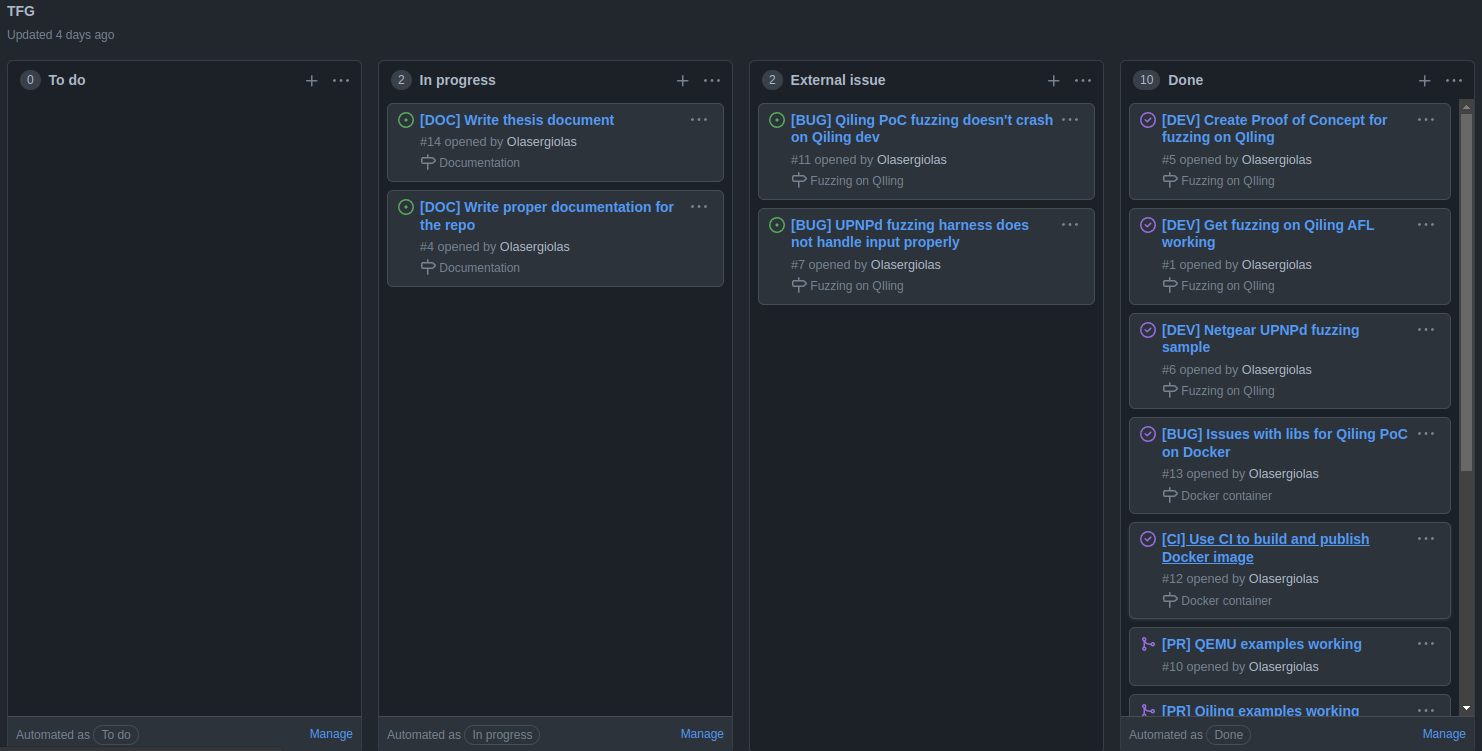
\includegraphics[scale=0.24]{kanban.png}}
    \caption{Funcionalidad de tablero Kanban de Github.}
\end{figure}

\begin{figure}
    \vspace*{-2.8in}
    \centering{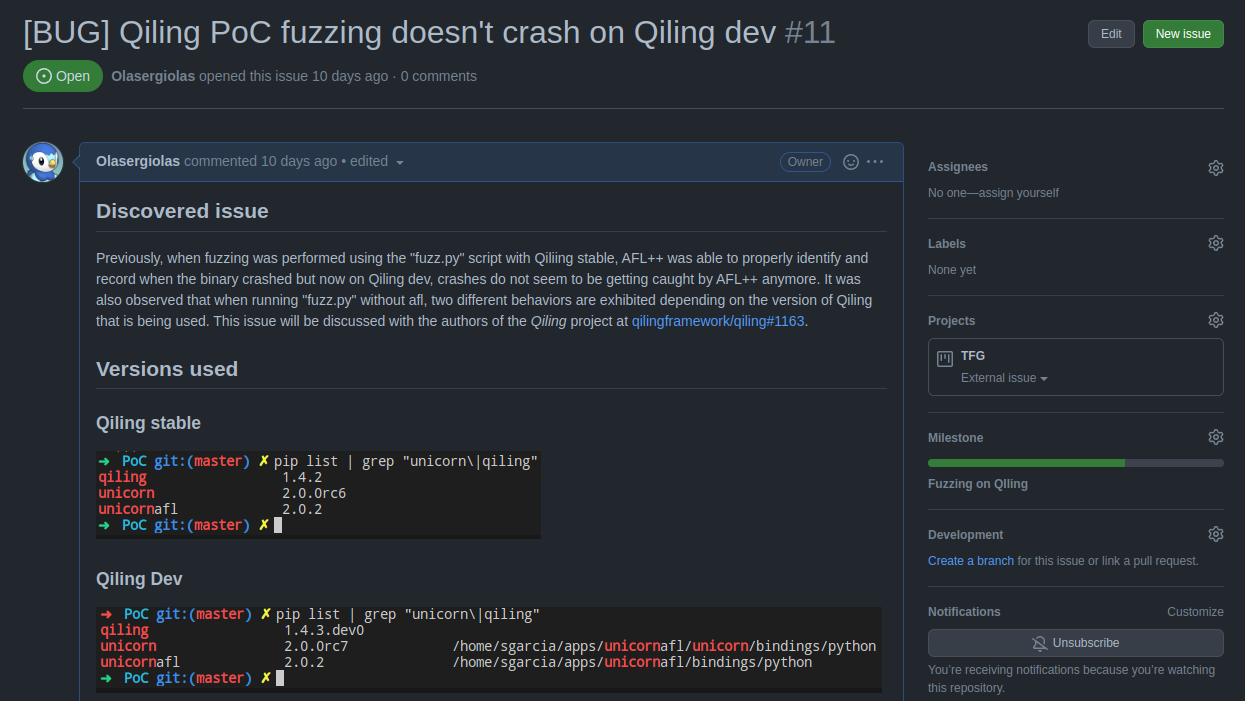
\includegraphics[scale=0.3]{issue.png}}
    \caption{Ejemplo de \href{https://github.com/Olasergiolas/TFG/issues/11}{issue} de reporte de bug en el repositorio del proyecto.}
\end{figure}

	% Estado del arte
	% 	1. Crítica al estado del arte
	% 	2. Propuesta
	\chapter{Estado del arte}
\label{estado_del_arte}

- Formas de hacerlo actualmente e Innovaciones
- Comentar varios proyectos
- Puntos positivos y negativos de todo

Desde el origen del fuzzing este ha sufrido avances.... tradicionalmente dumb fuzzing, luego 
paso a fuzzing que obtiene feedback de una manera u otra

Tradicionalmente, en el fuzzing orientado a dispositivos IoT no se han aplicando técnicas
específicas para este tipo de dispositivos, es decir, se asemejaba bastante al fuzzing de caja negra que 
comúnmente encontrado en aplicaciones como fuzzing de servicios web mediante la mutación de peticiones.
Este tipo de fuzzers caracterizados por no tener en cuenta el feedback del objetivo para la mutación de
inputs son conocidos como "dumb fuzzers" y presentan un flujo de ejecución simple el cual comienza 
con la mutación de un input válido,
a partir de ahí este input mutado es utilizado como parámetro del objetivo a fuzzear, si el 
objetivo (web, binario, etc.) produce un timeout o crashea el fuzzer registra el input que 
ha provocado este comportamiento y si el funcionamiento del objetivo es correcto, se ignora 
la información proporcionada por este y se vuelve a empezar. Dentro del dumb fuzzing hay también
distintos niveles de complejidad, algunos autores proponen fuzzers extremadamente básicos que 
llevan a cabo sus mutaciones de forma completamente aleatoria [TBD herramienta ejemplo] mientras 
que otros proponen utilidades como Radamsa [TBD insertar cita] que aún aplicando un enfoque de caja negra,
es capaz de inferir información del input original y utilizar heurísticas y patrones que son
modificables en tiempo de ejecución para conseguir una mayor tasa de éxito. [TBD ventajas y 
desventajas del dumb fuzzing, enganchas con las ventajas que supone el poder obtener feedback 
y comenta que esto es especialmente difícil en el fuzzing IoT]


[TBD Cuando se habla de fuzzing orientado a dispositivos IoT todas las técnicas y métodos para llevarlo 
a cabo suelen enfoque emulación, en hardware o híbrido]

	% Descripción del problema y hasta donde se llega
	\chapter{Descripción del problema}
\label{descripcion}
- Para comprender los problemas del fuzzing en IoT debemos primero tratar comprender el funcionamiento 
del fuzzing en general un poco más en profundidad ¿cómo funciona el fuzzing?.
- Para aplicar fuzzing en general necesitamos esto esto y lo otro.
- Al querer aplicarlo en IoT nos enfrentamos a X problemas (black-box, coverage, lentitud, estabilidad, 
emular de forma fiel al entorno original).
- Nombres de técnicas genéricas, sin especificar productos concretos como QEMU o Unicorn.	

	% Análisis del problema
	% 1. Análisis de requisitos
	% 2. Análisis de las soluciones
	% 3. Solucion propuesta
	% 4. Análisis de seguridad
	\chapter{Análisis del problema}
 \label{analisis}
 - Qué requisitos necesitamos cumplir
 - Analizar las posibles soluciones

	% Desarrollo bajo sprints: 
	% 	1. Permitir registros y login de usuarios
	% 	2. Desarrollo del sistema de incidencias
	% 	3. Desarrollo del sistema de denuncias administrativas y accidentes
	% 	4. Desarrollo del sistema de croquis
	%   5. Instalación de la aplicación de manera automática
	\chapter{Implementación}
\label{implementacion}

La implementación del software se ha dividido en hitos. Estos, han sido definidos en Github
y cada uno de ellos contiene un grupo de \textit{issues} que se corresponden con las distintas
mejoras que se han ido incorporando al software a lo largo de su desarrollo.\\



	% Conclusiones
	\chapter{Conclusiones y trabajos futuros}
\label{conclusiones}

	% Trabajos futuros
	
	\newpage
	\bibliography{bibliografia}
	\bibliographystyle{plain}
	
\end{document}

